\documentclass{polytech/polytech}
\usepackage{pdfpages}
% zone du préambule
\typereport{ppgldi4}

\reportyear{2017-2018}

\title{Création de fond de planning}
% https://gitlab.projectsforge.org/polytech/polytech/wikis/home

\student{Hanyuan}{Peng}{hanyuan.peng@etu.univ-tours.fr}
\student{Stéphane}{Deluce}{stephane.deluce@etu.univ-tours.fr}

\academicsupervisor[di]{Christophe}{Lenté}{christophe.lente@univ-tours.fr}

\resume{Le programme devra créer un fond de planning en Excel afin de faciliter la création des emplois	du temps. Grossièrement, le fond de de planning se présente comme un quadrillage avec en ligne les cours (CM, TD, TP) et en colonne les semaines. Des formules de calculs sont ajoutées à certaines cases afin de comptabiliser les heures placées. Le programme prendra en entrée un fichier excel (ou au pire csv) contenant une maquette et les enseignants affectés. Il fournira en sortie un fichier excel.}
\motcle{Java}
\motcle{Excel}
\motcle{Apache POI}

\abstract{The program will need to create an Excel planning fund to facilitate the creation of timetables. Roughly speaking, the planning background is presented as a grid with on-line courses (CM, TD, TP) and in columns during the weeks. Calculation formulas are added to certain boxes in order to count the hours placed. The program will take an excel (or at worst csv) file containing a mock-up and the affected teachers as input. It will output an excel file.}
\keyword{Java}
\keyword{Excel}
\keyword{Apache POI}


% zone du préambule
\begin{document}
	% zone du contenu du document
	\chapter{Introduction}
	\section{Présentation du projet}
	L’objectif de projet est de développer un programme qui devra créer un fond de planning en Excel afin de faciliter la création des emplois du temps.
	Grossièrement, le fond de de planning se présente comme un quadrillage avec en ligne les cours (CM, TD, TP) et en colonne les semaines.
	Des formules de calculs sont ajoutées à certaines cases afin de comptabiliser les heures placées.
	Le programme prendra en entrée un fichier excel (ou au pire csv) contenant une maquette et les enseignants affectés. Il fournira en sortie un fichier excel.
	
	\chapter{Environnement de développement}
	\section{Language de programmation}
	Nous avons utilisé Java (version 1.8) comme langage de programmation car il a une performance satisfaisante sur tous les systèmes et c'est aussi la dernière version stable.
	Nous avons choisi comme IDE Eclipse pour développer le programme, car c'est un outil que nous avions tous les deux déjà utilisé.
	Eclipse nous permet aussi simplement de mettre en place des tests unitaires, a l'aide de JUnit.
	%Nous pouvons faire le développement et aussi les tests unitaires simplement avec Eclipse et Java, de plus c'est avec cet outils que nous avions l'habitude de travailler.

	\section{Outils de gestion de projet}
	Nous avons mis en place un Git comme système de versionning, et nous avons fais le choix d'heberger notre code à l'aide de GitLab qui nous permet de faire des projets privés. GitLab nous permettais aussi de centraliser notre code à un même endroit.
	
	Notre projet utilisera des bibliothèques, pour simplifier la gestion des dépendances, nous avons fait le choix d'utiliser Maven qui est un gestionnaire de dépendances pour Java.

	Nous avons fais le choix d'utiliser Trello pour gestion les tâches de notre projet.
	Ca nous permet de voir les taches qu'ils nous reste à faire, sur quelles taches travail notre binome, etc ...
	
	ScreenShot trello

	\chapter{Étude de projet}
	\section{Analyse des besoins}
	Expliquer les fonctions principales du projets … (formules, mise en formes)

	\section{Spécifications Fonctionnelles}

	\section{Modélisation}
	Nous utilisons l'architecture MVC (Modèle-vue-contrôleur) pour notre projet. La partie contrôleur est utilisée pour lire les données d'entrée, analyser les donnée et générer le planning. La partie modèle est utilisée pour stoker les données qu'on a lit et qu'on utilisera pour le planning. La partie vue est utilisée pour permettre les utilisateurs saisissent les commandes.

	\subsection{UML}

	\subsection{Définitions des classes}

	\chapter{Planification}

	\section{Découpage en taches}

	\section{Répartition des tâches}

	Nous avons choisi de se diviser le travail par classes.
	Avec des points régulier pour expliquer l'avancé de notre travail, et partager nos remarques et
	interrogations

	\chapter{Implémentation}

	Expliquer notre choix, formules, documentation, ...

	\section{Organisation}

	\subsection{Organisation des fichiers}

	Nous avons commencé par développer les modèles, puis les contrôleurs pour finir avec la vue.
	Tests unitaires ont étés réalisés après l'écriture de chaques méthodes de chaques classes.

	\section{Tests et validation}
	\subsection{Résultat d'exécution}
	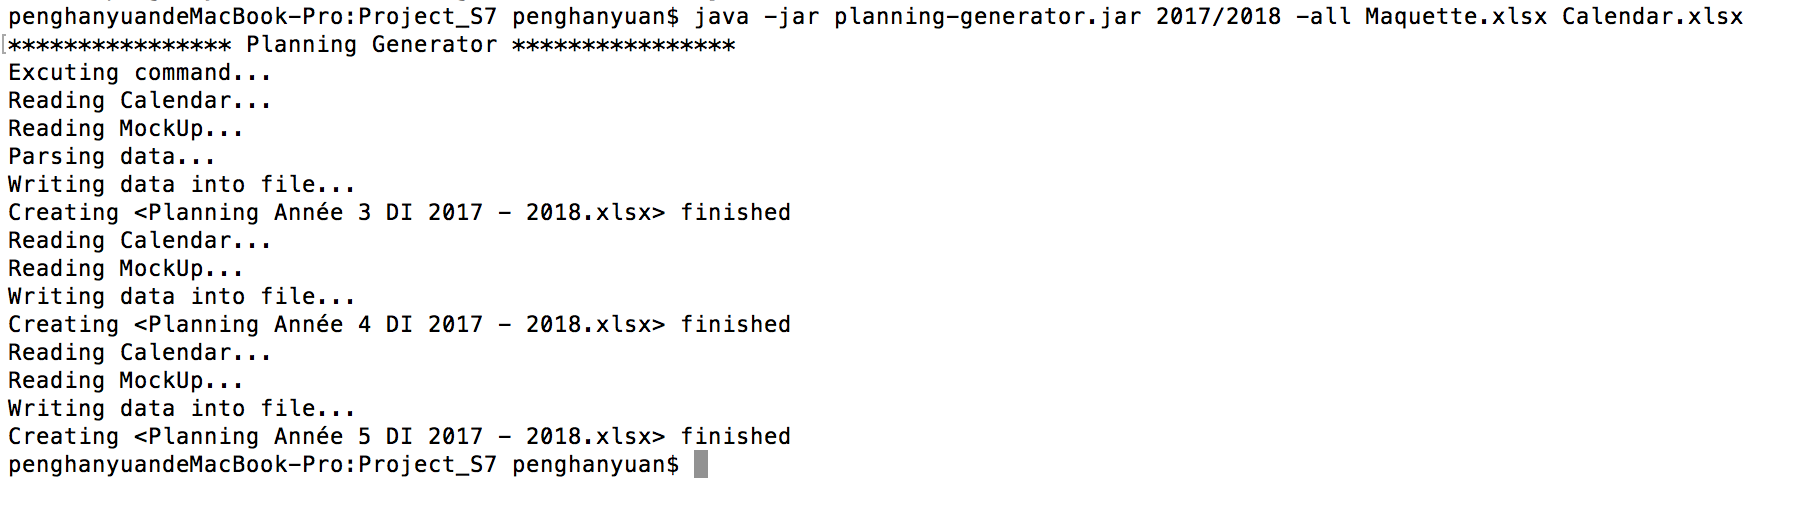
\includegraphics[width=\textwidth]{./img/excution_result.png}
	\section{Documentation}

	Classes documentés pour évolutivité, ...

	\chapter{Annexes}

	\section{Manuel d'utilisation}
	
\includepdf[pages=3-, offset=0 0]{../manuel.pdf}
\end{document}
